\documentclass[12pt]{article}
\usepackage[letterpaper]{geometry}
\usepackage{amsmath, amsthm, amssymb, amsfonts}
\usepackage{graphicx}
\usepackage{titling}
\usepackage{hyperref}
\newcommand{\subtitle}[1]{%
  \posttitle{%
    \par\end{center}
    \begin{center}\large#1\end{center}
    \vskip0.5em}%
}
\hypersetup{
    colorlinks=true,
    linkcolor=blue,
    filecolor=magenta,      
    urlcolor=blue,
} 
\urlstyle{same}
\title{CSE 150 - Operating Systems \\ Documentation \#3}
\subtitle{Spring 2018 - Lab 04 - Group 1}
\author{Avery Berchek, Aleksandr Brodskiy, David Cabral, Christopher DeSoto,\\Adiam G-Egzabher, Nanditha Embar, Christian Vernikoff}
\begin{document}
\maketitle
{\setlength{\parindent}{0cm}
\textbf{Outline}
\begin{enumerate}  
\item Documentation
\item Design Decisions
\item Testing/QA
\item Design Questions
\item Team Member Work-Log
\item Conclusion\\\\\\\\\\\\\\\\\\\\
\end{enumerate} 
}
{\setlength{\parindent}{0cm}
\textbf{Documentation} \\
\begin{center}Task I\end{center}
\paragraph{} The devised approach to developing an efficient, sound, and complete transport control 
    networking protocol was to dichotomize the implementation process into smaller abstractions such that
    the amalgamation of their respective functionalities would provide a successful 
    transmission control paradigm. In this manner the abstractions used to establish TCP are as follows:
    \begin{enumerate}
    \item The implementation of handling \textsc{accept} and \textsc{connect} syscalls. 
    \item The overriding of the \textsc{Read} function of \textsc{OpenFile} for the new \textsc{TransportFile} class. 
    \item The overriding of the \textsc{Write} function of \textsc{OpenFile} for the new \textsc{TransportFile} class. 
    \item The overriding \textsc{MailMessage} class to support TCP header fields.
    \item The implementation of handling connection teardown with the \textsc{close} function.
    \end{enumerate}
    \paragraph{} With these abstractions it becomes much easier to implement the deliverables of a successful TCP.
    Therefore the \textsc{accept} and \textsc{connect} syscalls were set$-$up with data structures associated with managing all the connections.
    Within this set$-$up the essence of the function \textsc{addConnection} is in creating a new hash element to be inserted to the connections hash structure to represent a new connection that is being created. 
    This is instantiated in the following data structure:
    \begin{center} \textsc{HashSet structure connections}; \end{center}
    The manipulation of the \textsc{connections} data structure by the \textsc{accept} and \textsc{connect} functions is modeled below in the following pseudo$-$code.
\begin{center} 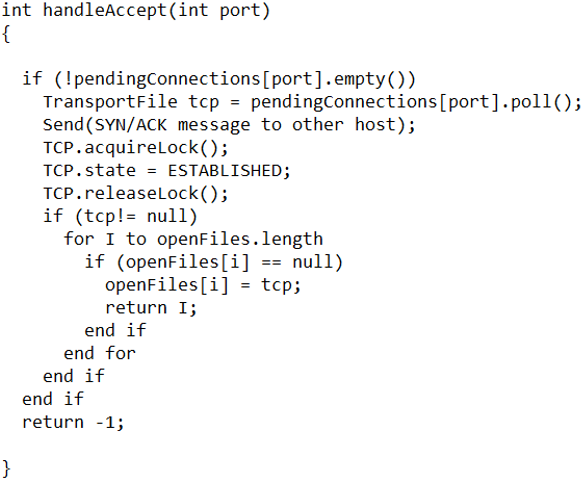
\includegraphics[width=110mm]{Accept.png} \end{center}
\begin{center} 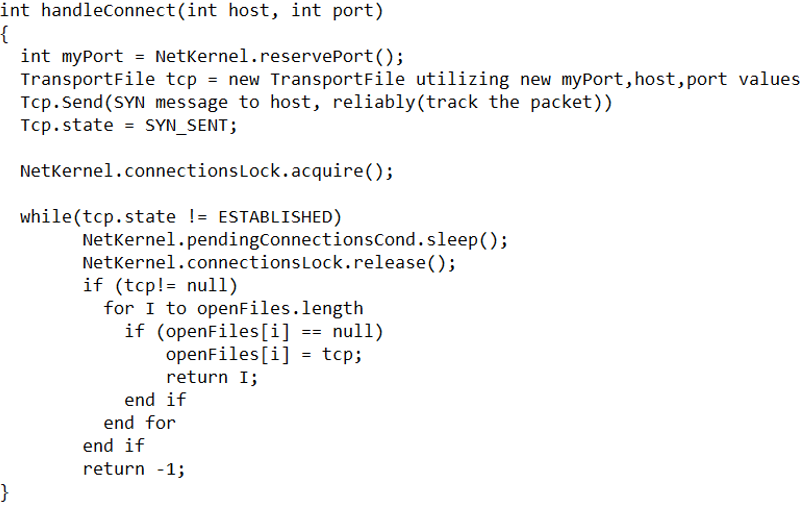
\includegraphics[width=130mm]{Connect.png} \end{center}
    \paragraph{} As is observable from the pseudo$-$code, the \textsc{accept} and \textsc{connect} functions enable the connections to TCP ports on the operating system
    through the two$-$way handshake \textsc{SYN} and \textsc{ACK} packet flag interchanges. However, it is also taken into consideration in the pseudo$-$code that there is an adjustment made to the packets being sent throughout the network that acknowledge what type of packet they are; for example, for an \textsc{ACK} packet flag the receive function would be modeled as follows. 
    The \textsc{connect} function, with respect to the accept 
    This functionality is very similar to \textsc{accept} with the preliminary discrepancy that it puts the thread that calls it to sleep, in this manner waiting for the \textsc{connect}ion to be established.
    The method in which threads are put to sleep is by each respective thread acquiring a static lock that is within the \textsc{NetKernel}.\textbf{\textit{java}} file, then a check is performed whether or not the connection has been established and if it hasn't then the threads are put to sleep on a condition variable. This allows multiple threads to be put to sleep to wait for a connection establishment. 
    Consequently, the functionality of the \textsc{Accept}/\textsc{Connect} in \textsc{Receive} is as follows:
    \begin{center} 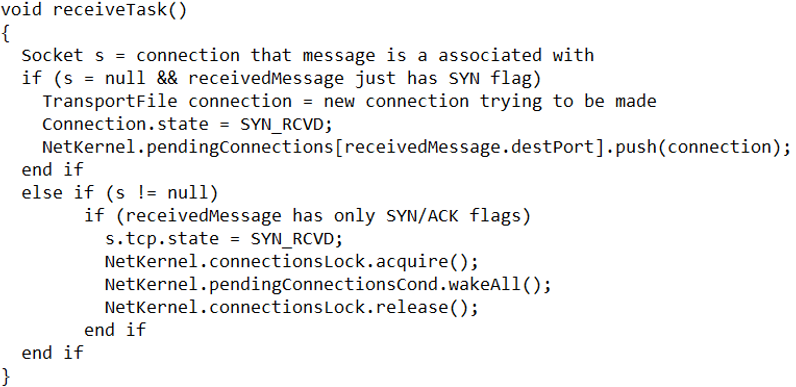
\includegraphics[width=125mm]{accpetConnectinReceive.png} \end{center}
    \paragraph{} The overriding of the \textsc{Read}/\textsc{Write} functions for the \textsc{NetKernel}.\textit{java} class was implemented with the following definitions for the \textsc{HashMap} data structure:
    \begin{center} \textsc{HashMap < String, Socket > currentConnections}; \end{center} 
    Where the \textsc{String} establishes both the local and remote ports as well as the remote machine address with the following variables:
    \begin{center} \textsc{localPort} \\ \textsc{remoteMachineAddress} \\ \textsc{remotePort} \end{center} 
    The \textsc{Semaphore} is introduced in the \textsc{HashMap} instantiation to notify when a packet has arrived.
    \paragraph{} In this manner the functionality for \textsc{notify}ing and \textsc{connect}ing are as follows:
    \begin{center} 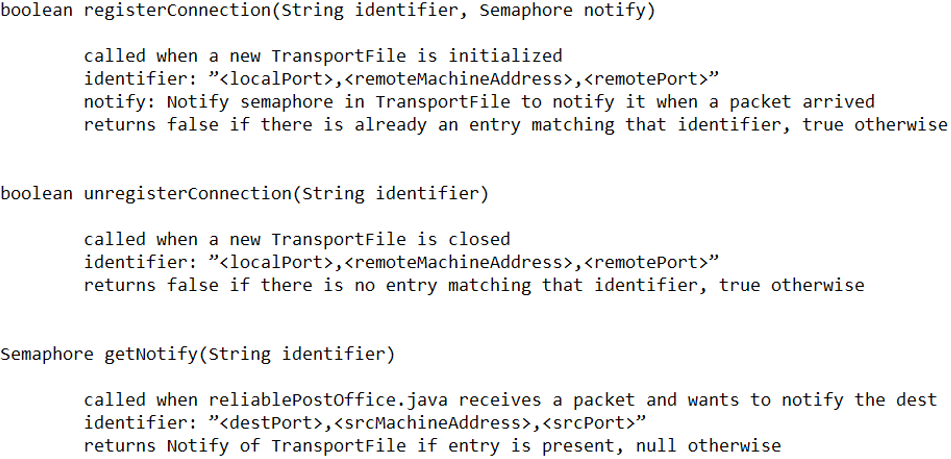
\includegraphics[width=140mm]{taskB.png} \end{center}
    \paragraph{} The implementation of the desired functionality for the \textsc{TransportFile}.\textit{java} class was developed in the internal classes:
    \begin{center} 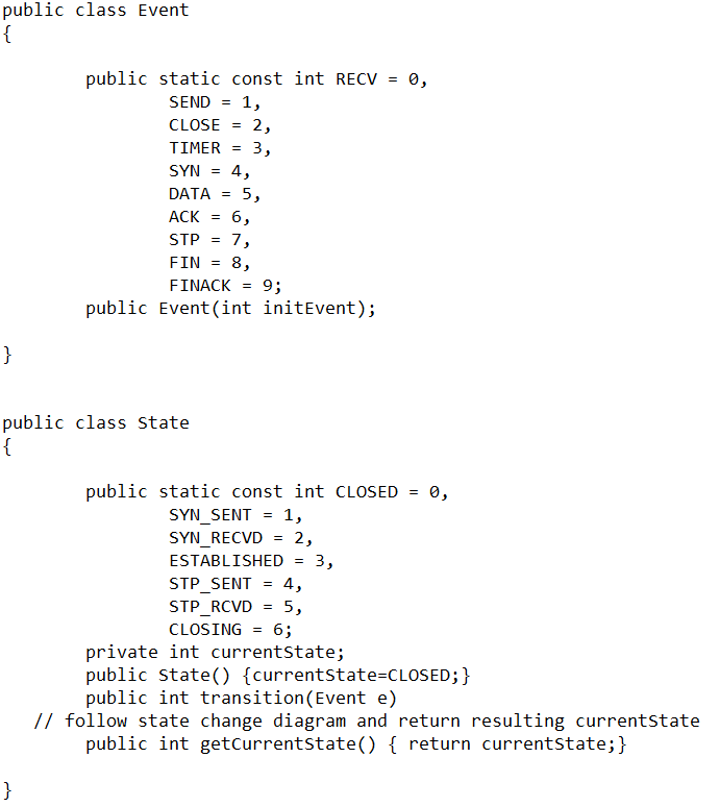
\includegraphics[width=95mm]{taskC.png} \end{center}
    With the following data structures:
\begin{center}
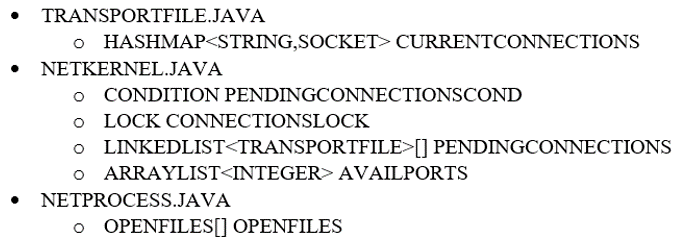
\includegraphics[width=120mm]{dataStructures.png}
\end{center} 
    \paragraph{} From the internal \textbf{\textit{java}} class, the implementation of \textsc{handleReceive}, \textsc{Read}, and \textsc{Write} was predominantly involved with the manipulation of \textsc{bytes}[] array in which
    the packets addressed and received were successfully transmitted.  \paragraph{}
    \begin{center} This is demonstrated in the following excerpt of code: \end{center}
    \begin{center} 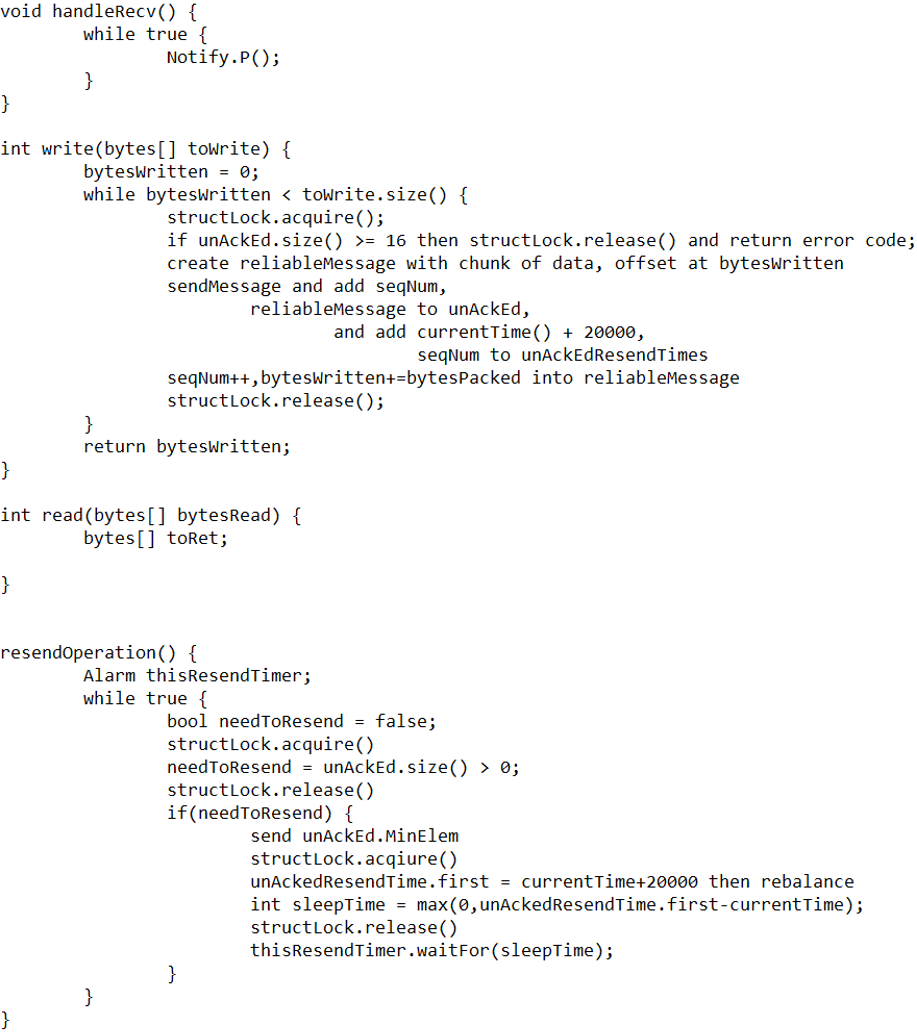
\includegraphics[width=130mm]{taskBC.png} \end{center}
    \paragraph{} Within the \textsc{while}(\textbf{\textit{true}}) loop of the \textsc{handleRecv} function, the \textsc{Notify.P}(); line signifies that a packet addressed
    to this was received, read the \textsc{reliableMessage} from \textsc{reliablePostOffice}, and follows the \textit{\textbf{nachos}} transport protocol for control packets; Otherwise the \textsc{structLock} is acquired and if this is an ACK then the corresponding entry in \textsc{unAckEd} and removed and unAckEdResendTimes then releases the \textsc{structLock} lock. 
    However, if this packet in transmission is categorized as data, then it is added to the \textsc{dataReceived} buffer. Then, the \textsc{structLock} lock is released to send an ACK. 
    \paragraph{} The overriding of the \textsc{MailMessage}.\textbf{\textit{java}} class to support the construction of transmission control packet header fields was done in the following manner with two constructor for the TCP.\textbf{\textit{java}} class:
    \begin{center} \textsc{TCP(\textbf{\textit{MailMessage}}, \textbf{\textit{seqNum}}, \textbf{\textit{ackNum}}, \textbf{\textit{controlSegment}});} \\ \textsc{TCP(\textbf{\textit{MailMessage}}, \textbf{\textit{seqNum}}, \textbf{\textit{ackNum}}, SYN, ACK, FIN, STP)}; \end{center}
    \begin{center} 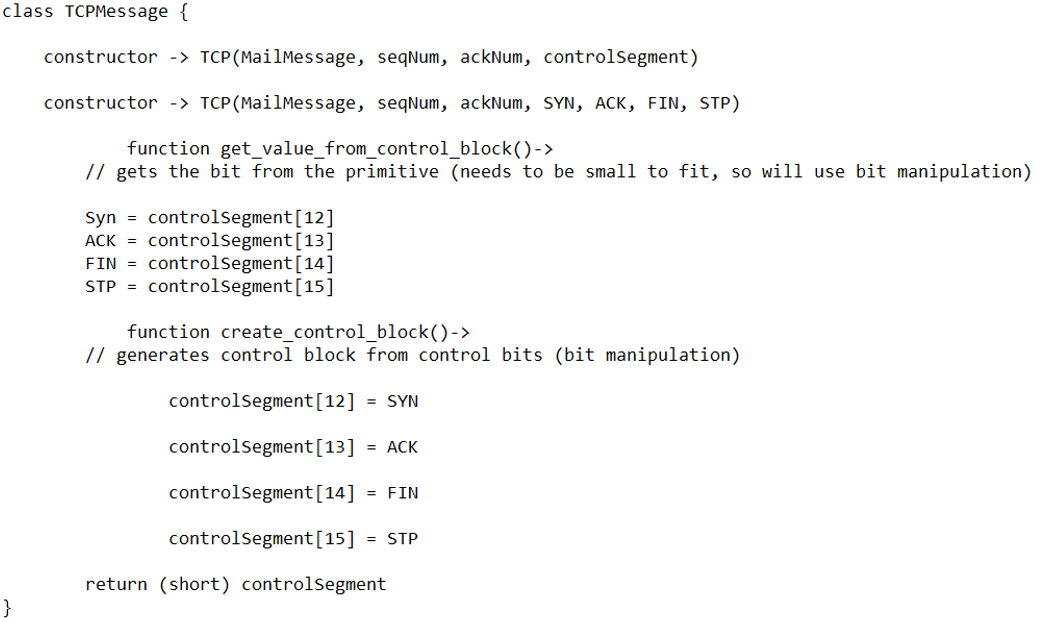
\includegraphics[width=150mm]{task1D.png} \end{center}
    The overloading of the TCP constructor allowed for the simplified addition of TCP based headers for reliability. 
    \paragraph{} Lastly, the implementation of the \textsc{close} function syscalls consummated the \textsc{TransportFile}.\textbf{\textit{java}} class
    as it facilitated a \textsc{clos}ing schematic for the connection and therefore provided the inverse two$-$handshake for the TCP teardown. Within this functionality
    when \textsc{close} is invoked, if the connection is still transmitting data then a \textsc{STP} packet will be sent to let the remote host know to stop sending data and just wait until the host that called close to stop sending data. 
    Once the data transmission is complete, and no longer acknowledged, then a \textsc{FIN} packet will be sent out to let the remote host know that the connection is closing. A \textsc{FIN}/\textsc{ACK} will be sent back from remote host so once received the connection will finally be \textsc{close}d and resources will be deallocated.  
    \paragraph{} This is demonstrated in the \textsc{close} in receive function:
\begin{center}
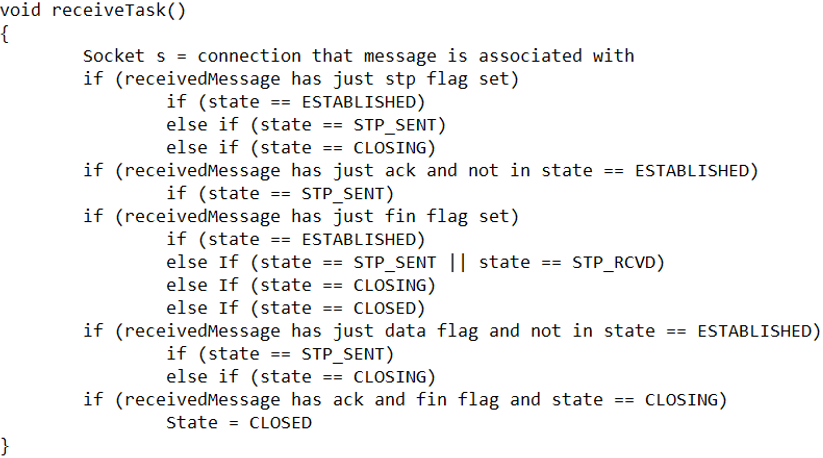
\includegraphics[width=110mm]{closeInReceive.png}
\end{center}
\paragraph{} The pseudo$-$code for the TCP teardown \textsc{close} function is as follows:
\begin{center}

\end{center} 
\begin{center}Task II\end{center}
\paragraph{} The implementation of a relay chat client$-$server application atop the implemented transmission control protocol was developed with functionality similar to that of aforementioned syscalls. 
\paragraph{} In this manner the primary objective of the chat application was to produce an N$-$way \textsc{chatServer}/\textsc{chat} deliverable. Therefore the initial approach was to model functionality resembling that of socket interfaces.
\paragraph{} It is observable from the pseudo$-$code that the \textsc{chatServer} program attempts to forward all incoming connections and throws an exception error to catch should there be any malfunctions.
Likewise, the functionality of the client node, is demonstrated in the pseudo$-$code excerpt below:
\begin{center} \includegraphics[width=100mm]{Chat.png} \end{center}
\paragraph{} With this implementation a clients can connect to the server at any time and disconnect at any time while the server handle clients entering and leaving the chat room at any point during the conversation.
Likewise, all users are able to view message contents in an identical format across all open connections. This feature is demonstrated in the following screenshot:
\begin{center}
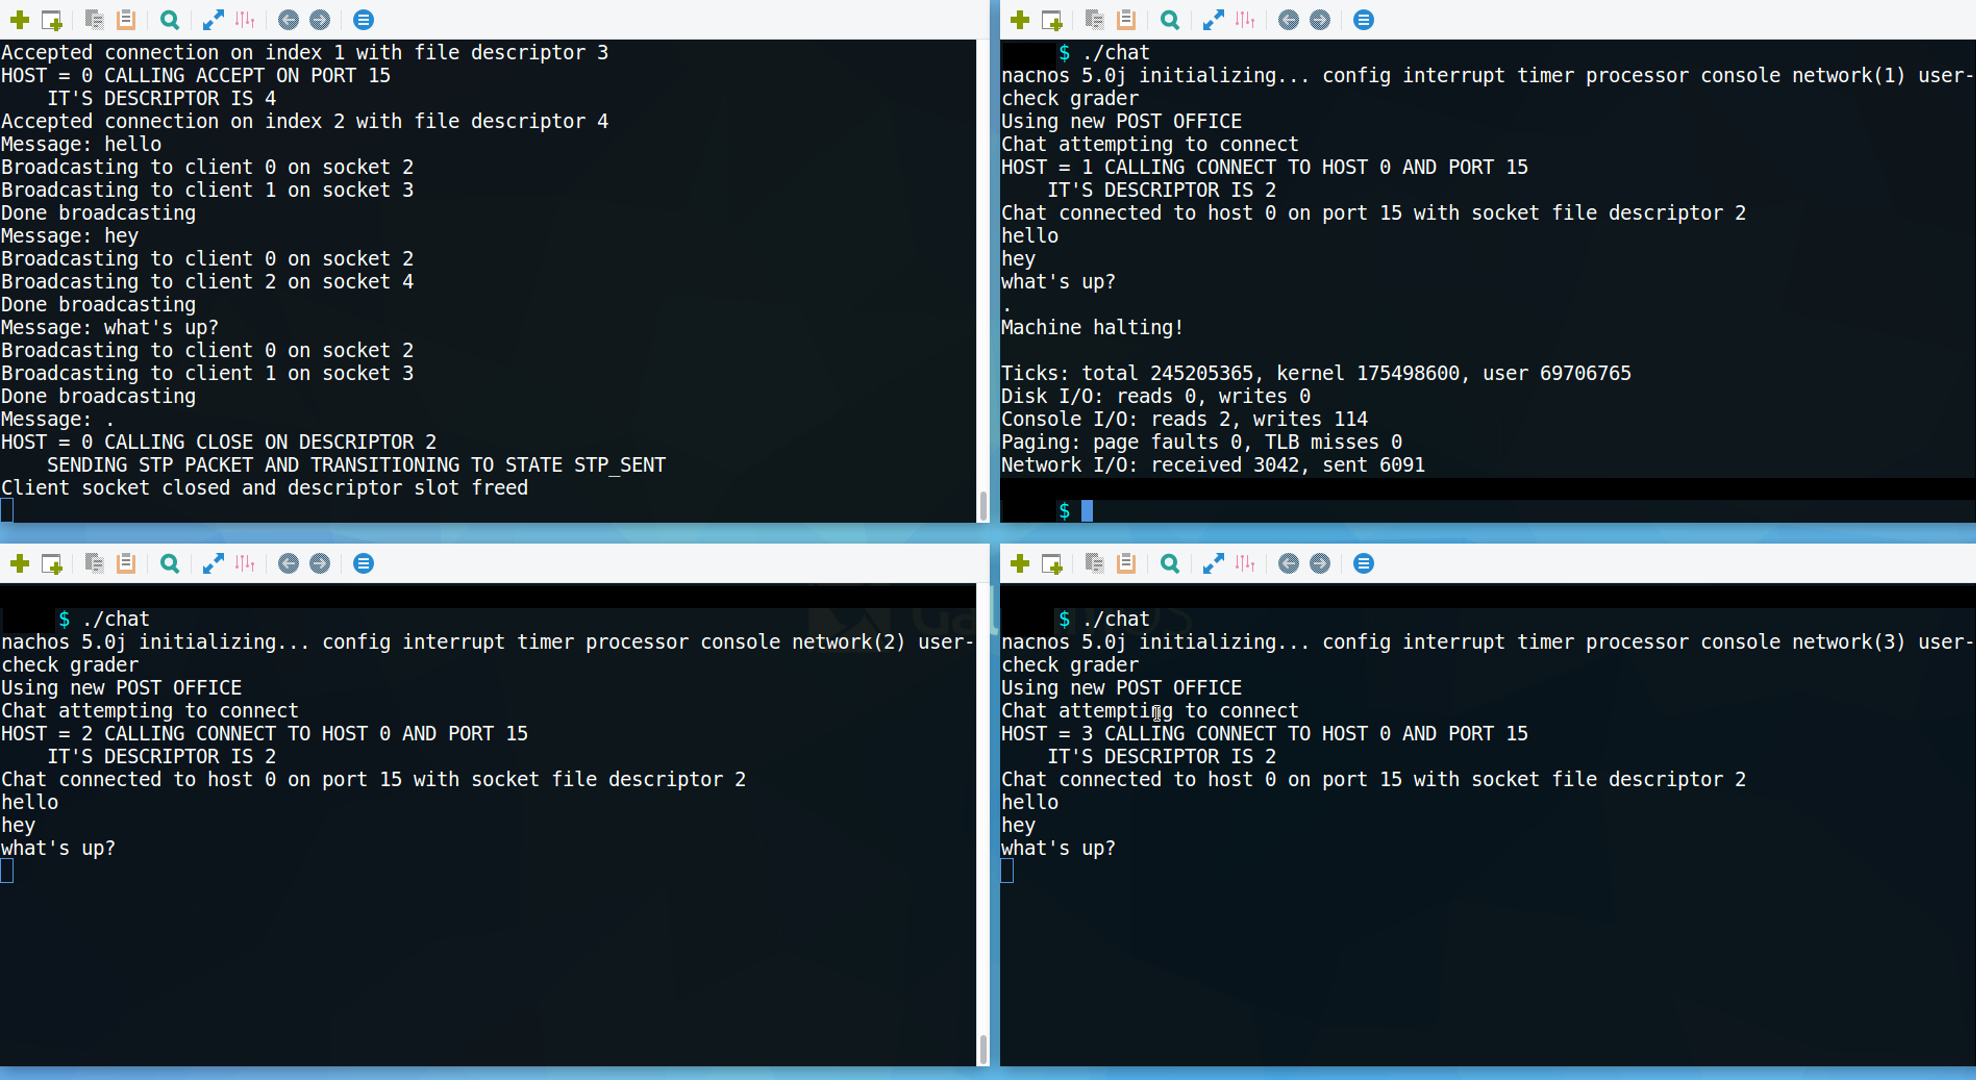
\includegraphics[width=160mm]{chatClientServer.png}
\end{center}
}
{\setlength{\parindent}{0cm}
\textbf{Design Decisions} \\
\paragraph{} * The chat client/server files are located within the \textsc{\textbf{\textit{test}}} directory.
\paragraph{} * Currently, 23/30 test cases pass. Redemption is established in the copious amounts of comments made in the submitted code.
\paragraph{} * Explanations of all primary testing strategies are explained in the following section.
\paragraph{} * Substantial time and resources were dedicated to debugging and quality control process.
\paragraph{} * A \textbf{\textit{byte}}$-$length field header was added to the TCP \textsc{Message} constructor.
\\\\
}
{\setlength{\parindent}{0cm}
\textbf{Testing/QA}\\
\begin{center}
Task I
\end{center}
\paragraph{} The following code addresses test cases related to the aforementioned abstractions
\begin{center} 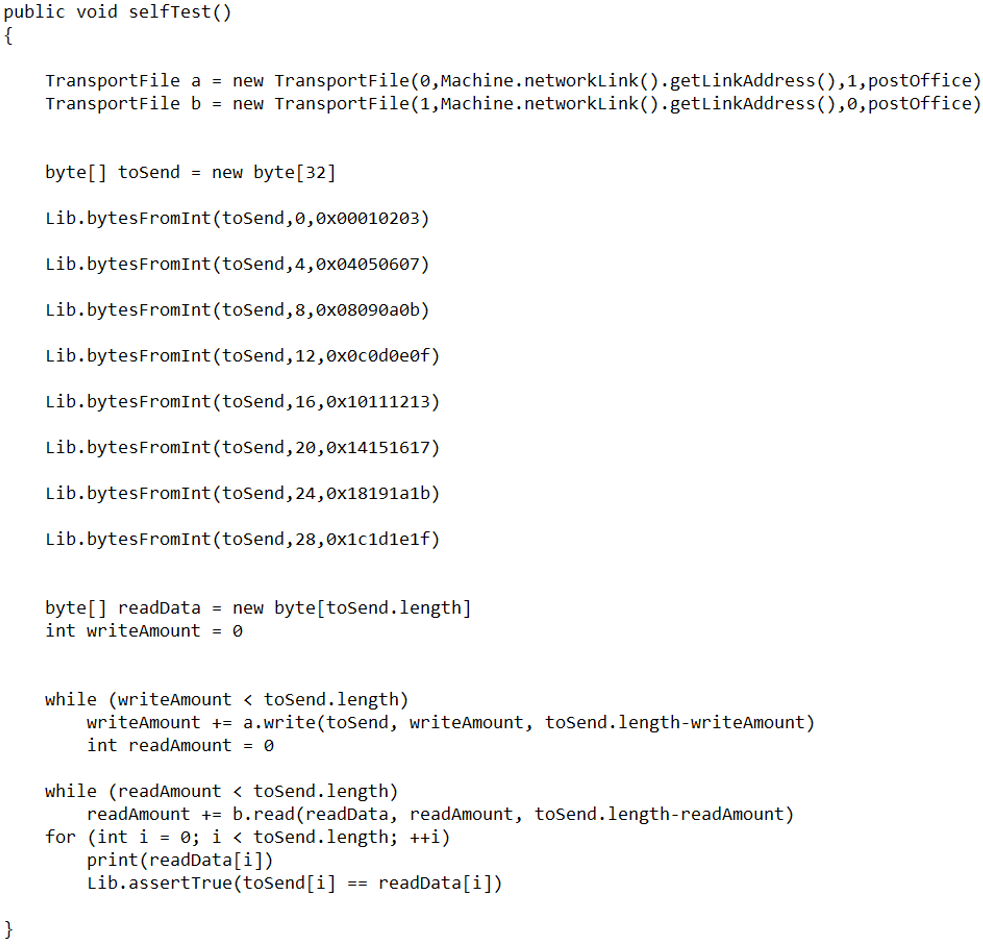
\includegraphics[width=150mm]{testCase1.png} \end{center}
\paragraph{} The above function, \textsc{selfTest}, essentially creates a buffer of bytes.
    The creation of such a buffer enables the connection of two sockets across each other on a link on the same machine.
    The idea of invoking a testing strategy in this manner was to isolate the \textsc{read} and \textsc{write} syscalls and test their respective functionality with regard to reliability for 
    the \textsc{read}ing and \textsc{writ}ing of data. Therefore the invocation of internal calls to the respective \textsc{TransportFile} class functions, as aforementioned \textsc{read} and \textsc{write},
    was able to isolate and determine their stochastic functionality to be reliable within an error tolerance of only 0.01 through the retransmission of packets.
\paragraph{} In order to model modern industrial programming paradigms, such as a minimally complete and verifiable example, reproductions of server errors were generated on local testing machines. This approached allowed for a more robust method of finding heisen$-$bugs and other difficult to contain, errors. Primarily, the \textsc{close} function which instantiated the TCP teardown.  
\paragraph{} Another testing strategy utilized for the verification of the \textsc{connect} function revolved around the instantiation of two machines. One machine would invoke the \textsc{connect} function and make sure that it got put to sleep by including a print statement at the end of the \textsc{connect} function to see if it would wait for connection establishment. Then, once \textsc{connect} was called, the \textsc{accept} function on the other machine would print to the console the statement included on the other machine. In this manner naively verifying the case that \textsc{connect} would wait for connection establishment.
\paragraph{} A strategy similar to this was utilized for testing reliability. The preliminary discrepancy in that case was to make sure that a \textsc{SYN} was transmitted multiple times until a \textsc{SYN/ACK} was received.  
\begin{center}
Task II
\end{center}
\paragraph{} In order to test chat string length we inputted strings of increasing sizes from 1 to 300. 
\begin{center}
``\textbf{\textit{f}}''\\
``\textbf{\textit{ffffffffff}}''\\
``\textbf{\textit{ffffffffffffffffffffffffffffffffffffffffffffffffffffffffffffffffffffffffffffffffffffffffffffffffffff}}''\\
etc...\\
\end{center}
\paragraph{} In doing so we observed that the \textit{printf} statement utilized from the given \textsc{printf.c} file has a maximum buffer size of 256 bytes. Therefore, given our implementation, the maximum chat message size is 256 bytes.
\paragraph{} The test for the server's client capacity was simple and involved opening eight chat clients communicating on a single server. Each client was tested and N-way communication was verified. This exceeded the project specification of at least 3 clients. Note: Our implemention supports up to 16 clients communicating on a single server.
\paragraph{} Client argument testing was slightly unconventional. The project specification did not specify any command-line arguments for the chat client, however, the system call, \textbf{\textit{connect(int host, int portNumber)}}, required the inclusion of the host socket. Our implementation, therefore, accepts a single integer via the command-line and assigns it to be passed as the host socket when the connect system call is made. In order to test this, \textsc{Machine.java} and \textsc{UserKernel.java} were modified and functionality for command-line arguments was implemented. Within \textsc{Machine.java}, a new method was created to return the process name and command-line arguments a string array:
\begin{center}
    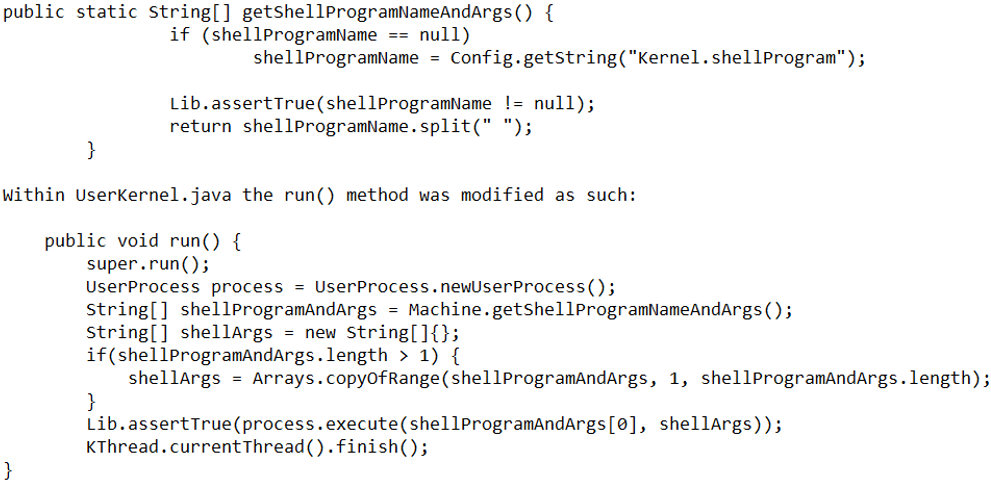
\includegraphics[width=160mm]{Task2Tests.png}
\end{center}
\paragraph{} This allowed command-line arguments to be passed when running the chat client (this argument specifies a host socket number of 0):
	\begin{center} \textsc{java nachos.machine.Machine -x 'chat.coff 0'} \end{center}
\paragraph{} In doing so, we we're able to verify our implemention. Note: The above code is not included in the final submission code and was implemented temporarily, strictly for testing purposes.
\paragraph{} Client disconnection was tested by passing the specified '.' message within the chat client. This was verified via printf statements from the server and clent. The clients were observed to send the disconnect message to the server and immediately exit. The server was observed to call the close() system call and assign -1 to the clients file descriptor, freeing the slot with in the array of clients to be used again should another client connect. \\\\
}
{\setlength{\parindent}{0cm}
\textbf{Team Member Work-Log}\\ \\
\textbf{\begin{center}\underline{Avery Berchek}\\DevOps Engineer\end{center}} 
\begin{itemize}
\item Designed and outlined the pseudo$-$code for \textsc{TransportFile} read/write and \textsc{PostOffice} manipulations.
\item Implemented the algorithmic functionality for read/write.
\item Primarily responsible for implementation of corner$-$case test cases.
\item Conducted and performed code reviews.
\end{itemize}
\textbf{\begin{center}\underline{Aleksandr Brodskiy}\\Project Manager\end{center}}  
\begin{itemize} 
\item Organized the \textit{sprints} and weekly meetings in accordance with the \textit{Agile/Scrum} project management methodology.
\item Delegated tasks and assigned roles for the Engineering Team as well as conducted the code reviews.
\item Outlined and participated in the design process associated with read/write.
\item Created and formatted the Design Documentation.
\item Managed all progress and operations of the Engineering Team in order to provide an efficient, robust, and optimal solution for a timely and submission.
\end{itemize}
\textbf{\begin{center}\underline{David Cabral}\\Design Engineer\end{center}} 
\begin{itemize}
\item Designed and outlined the pseudo$-$code for \textsc{Accept} \& \textsc{Connect}.
\item Implemented the algorithmic functionality for \textsc{Accept} \& \textsc{Connect}.
\item Implemented the algorithmic functionality for \textsc{Close} \& TCP teardown.
\end{itemize}
\textbf{\begin{center}\underline{Christopher DeSoto}\\Principal Engineer\end{center}}
\begin{itemize} 
\item Designed and outlined the pseudo$-$code for the network chat application.
\item Implemented the algorithmic functionality for the network chat application.
\end{itemize}
\textbf{\begin{center}\underline{Adiam G-Egzabher}\\Systems Engineer\end{center}} 
\begin{itemize}
\item Outlined and participated in the pseudo$-$code development associated with necessary adaptations to various file syscalls for \textsc{TransportFile}.
\item Participated in the design process and Testing/QA phase for Task I.
\end{itemize}
\textbf{\begin{center}\underline{Nanditha Embar}\\QA Engineer\end{center}} 
\begin{itemize}
\item Outlined and participated in the pseudo$-$code development associated with necessary adaptations to various file syscalls for \textsc{TransportFile}.
\item Participated in the design process and Testing/QA phase for Task II.
\end{itemize}
\textbf{\begin{center}\underline{Christian Vernikoff}\\Software Engineer\end{center}} 
\begin{itemize}
\item Designed and outlined the pseudo$-$code for the\textsc{MailMessage} inherited child class.
\item Implemented the algorithmic functionality for the override \textsc{MailMessage}.java class to include TCP header fields. 
\end{itemize}
}
{\setlength{\parindent}{0cm}
\textbf{\\\\\\Conclusion}
\paragraph{} In finishing this project algorithmic functionality of TCP (higher layer) syscalls was implemented along with a chat client/server application.
Within this implementation, the consummation of a network stack as present in modern day operating systems was developed.
\end{document} 
